\begin{figure}[htbp]
\centering
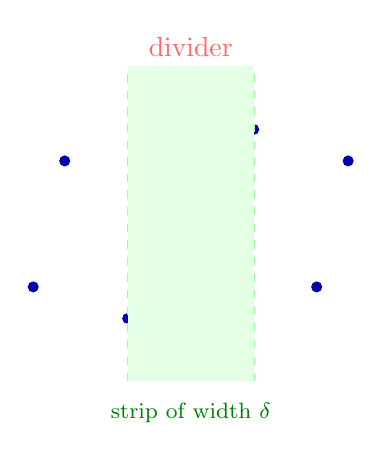
\begin{tikzpicture}[scale=0.8]
  \draw[red!60,thick,dashed] (3,-0.5)--(3,4.5) node[above] {divider};
  \fill[blue!70!black] (0.5,1) circle (2.5pt);
  \fill[blue!70!black] (1,3) circle (2.5pt);
  \fill[blue!70!black] (2,0.5) circle (2.5pt);
  \fill[blue!70!black] (2.5,2.5) circle (2.5pt);
  \fill[blue!70!black] (3.5,2) circle (2.5pt);
  \fill[blue!70!black] (4,3.5) circle (2.5pt);
  \fill[blue!70!black] (5,1) circle (2.5pt);
  \fill[blue!70!black] (5.5,3) circle (2.5pt);
  \draw[thick,orange] (2.5,2.5)--(3.5,2);
  \fill[orange] (2.5,2.5) circle (3pt);
  \fill[orange] (3.5,2) circle (3pt);
  \draw[green!40,thick,dashed] (2,-0.5)--(2,4.5);
  \draw[green!40,thick,dashed] (4,-0.5)--(4,4.5);
  \fill[green!10] (2,-0.5) rectangle (4,4.5);
  \node[font=\footnotesize,green!50!black] at (3,-1) {strip of width $\delta$};
\end{tikzpicture}
\caption{Closest pair: divide-and-conquer splits points along a vertical line. The closest pair may cross the dividing strip.}
\label{fig:closest_pair}
\end{figure}
